\section{Convex Optimisation}

\subsection{Convexity}

\subsubsection{Convex Functions}

\begin{definition*}[Convex Set]
    \label{def:convex-set}%
    A set \(S \subseteq \RR^n\) is \emph{convex}, if for any \(\vb{x}, \vb{y} \in S\) and \(\lambda \in \ccintv{0}{1}\), we have
    \[
        \lambda \vb{x} + \pqty{1 - \lambda} \vb{y} \in S.
    \]
\end{definition*}

\autoref{def:convex-set} says that a set is convex, if and only if the straight line segment that connects any two points is contained in the set.

\begin{definition*}[Convex Function]
    \label{def:convex-fn}%
    A function \(\functiondomain{f}{S}{\RR}\) is a \emph{convex} function, if \(S\) is convex, and for any \(\vb{x}, \vb{y} \in S\) and \(\lambda \in \ccintv{0}{1}\), we have
    \[
        f\pqty{\lambda \vb{x} + \pqty{1 - \lambda} \vb{y}} \leq \lambda f\pqty{\vb{x}} + \pqty{1 - \lambda} f\pqty{\vb{y}}.
    \]  
\end{definition*}

\begin{figure}[ht!]
    \centering
    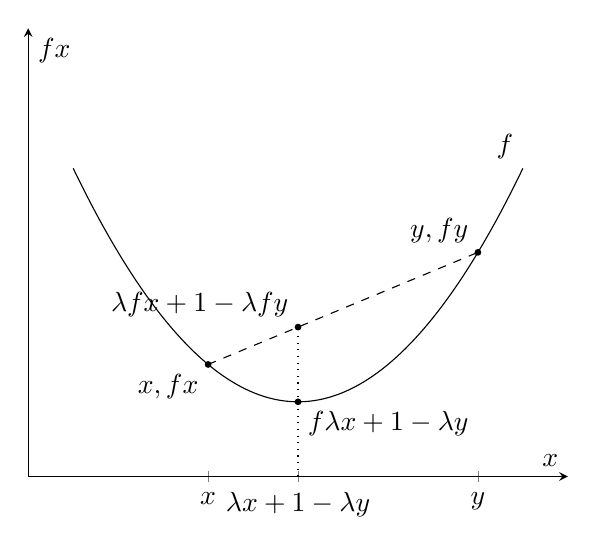
\begin{tikzpicture}
        \begin{axis}[
            axis lines = middle,
            xlabel = {\(x\)},
            ylabel = {\(f\pqty{x}\)},
            xmin = 0, xmax = 6,
            ymin = 0, ymax = 6,
            samples = 100,
            domain = 0.5:5.5,
            xtick = {2, 3, 5},
            xticklabels = {\(x\), \(\lambda x+\pqty{1-\lambda}y\), \(y\)},
            ytick = \empty
        ]

            \addplot[no marks] {0.5*(x-3)^2 + 1};
            \node[above left] at (axis cs:5.5,4.125) {\(f\)};

            \addplot[only marks, mark=*, mark size=1pt]
                coordinates {(2, 1.5) (5, 3)};

            \node[below left] at (axis cs:2, 1.5) {\(\pqty{x, f\pqty{x}}\)};
            \node[above left] at (axis cs:5, 3) {\(\pqty{y, f\pqty{y}}\)};

            \addplot[dashed] coordinates {(2, 1.5) (5, 3)};
            \addplot[only marks, mark=*, mark size=1pt]
                coordinates {(3, 2) (3, 1)};
            \node[above left] at (axis cs:3, 2) {\(\lambda f\pqty{x} + \pqty{1 - \lambda} f\pqty{y}\)};
            \node[below right] at (axis cs:3, 1) {\(f\pqty{\lambda x + \pqty{1 - \lambda} y}\)};

            \addplot[dotted] coordinates {(3, 0) (3, 2)};

        \end{axis}
    \end{tikzpicture}

    \caption{Convex Function}
    \label{fig:convex-fn}
\end{figure}

In other words, a convex function is a function whose chord lies above the curve.

\begin{remark}
    If \(-f\) is convex, then \(f\) is said to be concave. Linear functions are trivially both convex and concave.
\end{remark}

\subsubsection{First-Order Conditions}

\begin{figure}[ht!]
    \centering
    \begin{tikzpicture}
        \begin{axis}[
            axis lines = middle,
            xlabel = {\(x\)},
            ylabel = {\(f(x)\)},
            xmin = -1, xmax = 5,
            ymin = -2, ymax = 9,
            xtick = \empty,
            ytick = \empty,
            domain = 0:4,
            samples = 100,
            width = 10cm
        ]

            \addplot[no marks, thick, blue] {0.5*x^2};

            \addplot[only marks, mark=*, mark size = 1pt] coordinates {(1, 0.5) (2, 2) (3, 4.5)};

            \addplot[domain=0.25:4.5] {1 * (x - 1) + 0.5};
            \addplot[domain=0.4:4.2] {2 * (x - 2) + 2};
            \addplot[domain=0.5:4.1] {3 * (x - 3) + 4.5};
        \end{axis}
    \end{tikzpicture}

    \caption{Convex Function and its Tangents}
    \label{fig:convex-fn-tangents}
\end{figure}

We study in this section functions that are differentiable. By observing \autoref{fig:convex-fn-tangents}, it seems like the graph of a function always lie above its tangents, so we have
\[
    f\pqty{y} \geq f\pqty{x} + \pqty{y - x} f'\pqty{x}.
\]

In higher dimensions, we should have
\[
    f\pqty{\vb{y}} \geq f\pqty{\vb{x}} + \pqty{\vb{y} - \vb{x}} \transpose \grad f\pqty{\vb{x}}.
\]

\begin{theorem}[First-Order Condition]
    \label{thm:first-order-condition}%
    A differentiable function \(\functiondomain{f}{\RR^n}{\RR}\) is convex, if and only if for all \(\vb{x}, \vb{y} \in \RR^n\), we have
    \[
        f\pqty{\vb{y}} \geq f\pqty{\vb{x}} + \pqty{\vb{y} - 
        \vb{x}}\transpose \grad f\pqty{\vb{x}}.
    \]  
\end{theorem}

\begin{remark}
    If at \(x\), \(\grad f\pqty{x} = \vb{0}\), then \(x\) is a minimiser of \(f\).
\end{remark}

\begin{proof}
    We first suppose the function is convex. When \(n = 1\), we have
    \[
        f\pqty{x + t \pqty{y - x}} \leq \pqty{1 - t} f\pqty{x} + t f\pqty{y}
    \]
    for all \(t \in \ccintv{0}{1}\). This means
    \[
        f\pqty{y} \geq f\pqty{x} + \frac{f\pqty{x + t \pqty{y - x}} - f\pqty{x}}{t}.
    \]

    Taking the limit as \(t \to 0\),
    \[
        f\pqty{y} \geq f\pqty{x} + \pqty{y - x} f'\pqty{x}.
    \]

    To resolve the general case, for \(\vb{x}, \vb{y} \in \RR^n\), set
    \[
        g\pqty{t} = f\pqty{\pqty{1 - t} \vb{x} + t \vb{y}},
    \]  
    and \(g\) is a convex function with \(\functiondomain{g}{\ccintv{0}{1}}{\RR}\). Using the one-dimensional result, we have
    \[
        g\pqty{1} \geq g\pqty{0} + \pqty{1 - 0} g'\pqty{0}.
    \]

    Therefore.
    \[
        f\pqty{\vb{y}} \geq f\pqty{\vb{x}} + \grad f\pqty{\vb{x}} \transpose \pqty{\vb{y} - \vb{x}}.
    \]

    Now we prove the converse. Set
    \[
        \vb{x}_t = \pqty{1 - t} \vb{x} + t\vb{y}.
    \]

    First-order conditions imply that
    \begin{align*}
        f\pqty{\vb{x}} &\geq f\pqty{\vb{x}_t} + \grad f\pqty{\vb{x}_t} \transpose \pqty{\vb{x} - \vb{x}_t}, \\
        f\pqty{\vb{y}} &\geq f\pqty{\vb{x}_t} + \grad f\pqty{\vb{x}_t} \transpose \pqty{\vb{y} - \vb{x}_t}.
    \end{align*}

    Multiplying the first inequality by \(\pqty{1 - t}\) and the second by \(t\), and adding together, we have
    \[
        \pqty{1 - t} f\pqty{\vb{x}} + t f\pqty{\vb{y}} \geq f\pqty{\vb{x}_t} + 0 = f\pqty{\pqty{1 - t} \vb{x} + t \vb{y}}.
    \]
\end{proof}

\subsubsection{Second-Order Conditions}

We return to \autoref{fig:convex-fn-tangents}. We note that it seems that the slope of the gradient is increasing, so it means that \(f'' \geq 0\). But we shall generalise this to higher dimensions. For this, we recall the \emph{Hessian matrix}
\[
    \bqty{\grad^2 f\pqty{\vb{x}}}_{ij} = \pdv{f\pqty{\vb{x}}}{x_i}{x_j}.
\]

Recall that the one-dimensional Taylor series takes the form
\[
    f\pqty{y} = f\pqty{x} + \pqty{y - x} f'\pqty{x} + \frac{\pqty{y - x}^2}{2} f''\pqty{x} + \cdots
\]
and similarly, in the \(n\)-dimensional case, the Taylor series will have the form
\[
    f\pqty{\vb{y}} = f\pqty{\vb{x}} + \pqty{\vb{y} - \vb{x}}\transpose \grad f\pqty{\vb{x}} + \frac{1}{2} \pqty{\vb{y} - \vb{x}}\transpose \grad^2 f\pqty{\vb{x}} \pqty{\vb{y} - \vb{x}} + \cdots
\]

The proof is simple. If we apply the one-dimensional Taylor series to the function
\[
    g\pqty{t} = f\pqty{\vb{x} + \pqty{\vb{y} - \vb{x}} t},
\]
then
\[
    g\pqty{1} = g\pqty{0} + g'\pqty{0} + \frac{1}{2} g''\pqty{0} + \cdots
\]
so
\[
    f\pqty{\vb{y}} = f\pqty{\vb{x}} + \grad f\pqty{x} \transpose \pqty{\vb{y} - \vb{x}} + \frac{1}{2} \pqty{\vb{y} - \vb{x}} \transpose \grad^2 f\pqty{x} \pqty{\vb{y} - \vb{x}}.
\]

\begin{theorem}[Second-Order Condition]
    \label{thm:second-order-condition}%
    A twice-differentiable function function \(\functiondomain{f}{\RR^n}{\RR}\) is convex, if and only if
    \[
        \grad^2 f\pqty{x} \posDefEq 0
    \]
    for all \(x \in \RR^n\).
\end{theorem}

\begin{remark}
    We say a symmetric \(n\)-dimensional matrix \(\vb{A}\) is \emph{positive semi-definite}, denoted \(\vb{A} \posDefEq 0\), if
    \[
        \vb{x}\transpose \vb{A} \vb{x} \geq 0
    \]
    for all \(\vb{x} \in \RR^n\). Equivalently, all \(n\) eigenvalues of \(\vb{A}\) are non-negative.
\end{remark}

\begin{proof}[(One Direction Only)]
    We prove convexity from positive semi-definiteness. For any \(\vb{x}\) and \(\vb{y}\), we have for some \(\vb{z} \in \RR^n\) (by the intermediate value theorem),
    \begin{align*}
        f\pqty{\vb{y}} &= f\pqty{\vb{x}} + \grad f\pqty{\vb{x}} \transpose \pqty{\vb{y} - \vb{x}} + \frac{1}{2} \pqty{\vb{y} - \vb{x}} \transpose \grad^2 f\pqty{\vb{z}} \pqty{\vb{y} - \vb{x}} \\
        &\geq f\pqty{\vb{x}} + \grad f\pqty{\vb{x}} \transpose \pqty{\vb{y} - \vb{x}}
    \end{align*}

    This implies the first-order condition, so by \autoref{thm:first-order-condition}, \(f\) is convex.
\end{proof}

\subsection{Gradient Descent Algorithm}

We observe that
\[
    f\pqty{\vb{y}} \approx f\pqty{\vb{x}} + \grad f\pqty{\vb{x}} \transpose \pqty{\vb{y} - \vb{x}}.
\]

Say we have
\[
    \vb{y} - \vb{x} = - \epsilon \grad f\pqty{\vb{x}}
\]
where \(0 < \epsilon \ll 1\) is small. Then we have
\begin{align*}
    f\pqty{\vb{y}} &\approx f\pqty{\vb{x}} + \grad f\pqty{\vb{x}} \transpose \pqty{- \epsilon \grad f \pqty{\vb{x}}} \\
    &= f\pqty{\vb{x}} - \epsilon \norm{\grad f\pqty{\vb{x}}}^2.
\end{align*}

This leads to the gradient descent algorithm, as described in \autoref{alg:gradient-descent}.

\begin{algorithm}[htp!]
    \caption{Gradient Descent Algorithm}\label{alg:gradient-descent}%
    \begin{algorithmic}
        \Procedure{GradientDescent}{\(f, \vb{x}_0\)}
        \State \(t \gets 0\)
        \Repeat
            \State \(\vb{v}_t \gets - \grad f\pqty{\vb{x}_t}\)
            \State Choose Step Size \(\eta_t > 0\)
            \State \(\vb{x}_{t + 1} \gets \vb{x}_t + \eta_t \vb{v}_t\)
            \State \(t \gets t + 1\)
        \Until{Certain Stopping Criteria(s)}
        \EndProcedure
    \end{algorithmic}
\end{algorithm}

\begin{remark}
    The stopping criteria(s) can be, for example, when out computing power runs out, or the gradient is very small.
\end{remark}

We note that the gradient descent algorithm could fail: if the step size is too large, we might not necessarily reach the minimum, for example, we overshoot if the function is very steep. Similar issues appear when the step size is too small, for example, it will take very long to reach the minimum if the function is very flat.

Therefore, we restrict our class of functions.

\subsubsection{Smoothness and Strong Convexity}

\begin{definition}[\(\alpha\)-strong convexity, \(\beta\)-smooth]
    \label{def:alpha-sc-beta-smooth}%
    Let \(\alpha, \beta > 0\). A twice-differentiable function \(\functiondomain{f}{\RR^n}{\RR}\) is \emph{\(\beta\)-smooth} if \(\grad^2 f\pqty{\vb{x}} \negDefEq \beta \identityM\) for all \(\vb{x} \in \RR^n\); and is \emph{\(\alpha\)-strongly convex} if \(\grad^2 f\pqty{\vb{x}} \posDefEq \alpha \identityM\) for all \(\vb{x} \in \RR^n\).
\end{definition}

\begin{remark}
    We say two matrices \(\vb{A} \negDefEq \vb{B}\), if \(\vb{B} - \vb{A} \posDefEq 0\), i.e., \(\vb{B} - \vb{A}\) is a positive semi-definite matrix. This implies \(\vb{x}\transpose \vb{A} \vb{x} \leq \vb{x} \transpose \vb{B} \vb{x}\) for all \(\vb{x} \in \RR^n\).
\end{remark}

In other words, this condition states that the eigenvalues are at most \(\beta\), or at least \(\alpha\). Upper bounding by \(\beta\) rules out very steep functions, and lower bounding by \(\alpha\) rules out very flat functions.

\begin{theorem}[Second-Order (Quadratic) Bounds]
    \label{thm:second-order-quadratic-bounds}%
    Let \(\functiondomain{f}{\RR^n}{\RR}\) be twice-differentiable and \(\vb{x}, \vb{y} \in \RR^n\).

    \begin{itemize}
        \item If \(f\) is \(\beta\)-smooth, then
        \[
            f\pqty{\vb{y}} \leq f\pqty{\vb{x}} + \grad f\pqty{\vb{x}}\transpose \pqty{\vb{y} - \vb{x}} + \frac{\beta}{2} \norm{\vb{y} - \vb{x}}^2.
        \]

        \item If \(f\) is \(\alpha\)-strongly convex, then
        \[
            f\pqty{\vb{y}} \geq f\pqty{\vb{x}} + \grad f\pqty{\vb{x}}\transpose \pqty{\vb{y} - \vb{x}} + \frac{\alpha}{2} \norm{\vb{y} - \vb{x}}^2.
        \]
    \end{itemize}
\end{theorem}

We are essentially bounding the function \(f\) between two quadratics -- the \(\beta\) as an upper bound, and the \(\alpha\) as a lower bound -- and quadratic functions are easier to understand!

\begin{proof}
    We use the multivariate Taylor series expansion. Expanding around \(\vb{x}\), we have
    \[
        f\pqty{\vb{y}} = f\pqty{\vb{x}} + \grad f\pqty{\vb{x}} \transpose \pqty{\vb{y} - \vb{x}} + \frac{!}{2} \pqty{\vb{y} - \vb{x}}\transpose \grad^2 f\pqty{\vb{z}} \pqty{\vb{y} - \vb{x}}
    \]
    where \(\vb{z}\) is some point on the line segment joining \(\vb{x}\) and \(\vb{y}\).

    Now, observe that if \(f\) is \(\beta\)-smooth,
    \[
        \frac{1}{2} \pqty{\vb{y} - \vb{x}}\transpose \grad^2 f\pqty{\vb{x}} \pqty{\vb{y} - \vb{x}} \leq \frac{1}{2} \pqty{\vb{y} - \vb{x}}\transpose \pqty{\beta \identityM} \pqty{\vb{y} - \vb{x}} = \frac{\beta}{2} \norm{\vb{y} - \vb{x}}^2,
    \]
    and similarly, if \(f\) is \(\alpha\)-strongly convex,
    \[
        \frac{1}{2} \pqty{\vb{y} - \vb{x}}\transpose \grad^2 f\pqty{\vb{x}} \pqty{\vb{y} - \vb{x}} \geq \frac{1}{2} \pqty{\vb{y} - \vb{x}}\transpose \pqty{\alpha \identityM} \pqty{\vb{y} - \vb{x}} = \frac{\alpha}{2} \norm{\vb{y} - \vb{x}}^2.
    \]
\end{proof}

Two very important corollaries are as follows.

\begin{corollary}[Sufficiently Small Step Size]
    \label{cor:grad-descent-beta-bound}%
    If \(f\) is \(\beta\)-smooth, then
    \[
        f\pqty{\vb{x} - \frac{1}{\beta} \grad f\pqty{\vb{x}}} \leq f\pqty{\vb{x}} - \frac{1}{2 \beta} \norm{\grad f\pqty{\vb{x}}}^2.
    \]
\end{corollary}

This basically states that if our function is sufficiently flat (\(\beta\)-smooth) (i.e. its sharpness is controlled), then a step size of \(\flatfrac{1}{\beta}\) is small enough to ensure we are always descending (and not overshoot)

\begin{proof}
    Substitute \(\vb{y} = \vb{x} - \flatfrac{\grad f\pqty{\vb{x}}}{\beta}\) into \autoref{thm:second-order-quadratic-bounds}.
\end{proof}

\begin{corollary}[Upper Bound on Difference to Minimum]
    \label{cor:grad-descent-alpha-bound}%
    Let \(f\) is \(\alpha\)-strongly convex, and let \(f\pqty{\vb{x}^{\ast}}\) be the minimum of \(f\). Then for any \(\vb{x}\), we have
    \[
        f\pqty{\vb{x}^{\ast}} \geq f\pqty{\vb{x}} - \frac{1}{2 \alpha} \norm{\grad f\pqty{\vb{x}}}^2.
    \]

    Equivalently,
    \[
        f\pqty{\vb{x}} - f\pqty{\vb{x}^{\ast}} \leq \frac{1}{2 \alpha} \norm{\grad f\pqty{\vb{x}}}^2.
    \]
\end{corollary}

This basically states that if our function is sufficiently steep (\(\alpha\)-strongly convex) (i.e. its flatness is controlled), then we have a bound on the distance (measured in the function value) to the minimum. If \(\norm{\grad f\pqty{\vb{x}}}^2 \leq 2 \alpha \epsilon\), then \(\vb{x}\) is optimal up to \(\epsilon\) error. This allows us to control the error, even for very flat functions.

\begin{proof}
    By \autoref{thm:second-order-quadratic-bounds}, we have
    \[
        f\pqty{\vb{y}} \geq f\pqty{\vb{x}} + \grad f\pqty{\vb{x}}\transpose \pqty{\vb{y} - \vb{x}} + \frac{\alpha}{2} \norm{\vb{y} - \vb{x}}^2.
    \]

    We take the minimum over \(\vb{y}\) on both sides. Then
    \[
        f\pqty{\vb{x}^{\ast}} \geq \min_{\vb{y} \in \RR^n} \bqty{f\pqty{\vb{x}} + \grad f\pqty{\vb{x}}\transpose \pqty{\vb{y} - \vb{x}} + \frac{\alpha}{2} \norm{\vb{y} - \vb{x}}^2}.
    \]

    Differentiating with respect to \(\vb{y}\) on the right-hand side gives
    \[
        \grad f\pqty{\vb{x}} + \alpha \pqty{\vb{y} - \vb{x}}
    \]
    as the gradient, and setting this equal to zero gives
    \[
        \vb{y} = \vb{x} - \frac{1}{\alpha} \grad f\pqty{\vb{x}}.
    \]

    Call this \(\vb{y}^{\ast}\). Plug this back into \autoref{thm:second-order-quadratic-bounds}, we have
    \[
        f\pqty{\vb{x}^{\ast}} \geq f\pqty{\vb{x}} - \frac{1}{2\alpha} \norm{\grad f\pqty{\vb{x}}}^2
    \]
    as desired.
\end{proof}

\subsubsection{Convergence of Gradient Descent}

\begin{theorem}[Exponentially-Fast Bound of Distance to Minimum]
    \label{thm:exp-bound-dist-minimum}%
    Let \(f\) be \(\alpha\)-strongly convex and \(\beta\)-smooth. Suppose \(f\) is minimised at \(\vb{x}^{\ast}\). Then gradient descent with a fixed step size of \(\eta_t = \frac{1}{\beta}\) satisfies
    \[
        f\pqty{\vb{x}_T} - f\pqty{\vb{x}^{\ast}} \leq \pqty{1 - \frac{\alpha}{\beta}}^{T} \pqty{f\pqty{\vb{x}_0} - f\pqty{\vb{x}^{\ast}}} \leq e^{- \flatfrac{\alpha T}{\beta}} \pqty{f\pqty{\vb{x}_0} - f\pqty{\vb{x}^{\ast}}}.
    \]
\end{theorem}

\begin{remark}
    The second inequality simply comes from \(e^{-x} \geq 1 - x\).
\end{remark}

In other words, taking
\[
    T \geq \frac{\beta}{\alpha} \log \pqty{\frac{f\pqty{\vb{x}_0} - f\pqty{\vb{x}^{\ast}}}{\epsilon}}
\]
gives an \(\epsilon\)-optimal point. This type of convergence is called \emph{linear convergence} in optimisation literature -- this is a good benchmark, since \(\log\) is `like a constant' in computer science, so if you have an algorithm that converges like \(\log\), then it is really good.

\begin{proof}
    Observe that
    \begin{align*}
        f\pqty{\vb{x}_{t + 1} - \vb{x}^{\ast}} &\leq f\pqty{\vb{x}_t} - f\pqty{\vb{x}^{\ast}} - \frac{1}{2\beta} \norm{\grad f\pqty{\vb{x}_t}}^2 && \text{\autoref{cor:grad-descent-beta-bound}} \\
        &\leq f\pqty{\vb{x}_t} - f\pqty{\vb{x}^{\ast}} - \frac{\alpha}{\beta} \pqty{f\pqty{\vb{x}_t} - f\pqty{\vb{x}^{\ast}}} && \text{\autoref{cor:grad-descent-alpha-bound}} \\
        &= \pqty{1 - \frac{\alpha}{\beta}} \pqty{f\pqty{\vb{x}_t} - f\pqty{\vb{x}^{\ast}}}.
    \end{align*}

    This reduces to our desired result by telescoping.
\end{proof}

\begin{example}
    Suppose in \(\RR^2\), let
    \[
        f\pqty{\vb{x}} = \frac{1}{2} \pqty{x_1^2 + 100 x_2^2}.
    \]

    Then
    \[
        \grad^2 f\pqty{\vb{x}} = \bmqty{\dmat{1,100}}.
    \]

    Then \(\alpha = 1\) and \(\beta = 100\), but
    \[
        1 - \frac{\alpha}{\beta} = 0.99
    \]
    is very close to \(1\). This number \(\flatfrac{\alpha}{\beta}\) is too small -- and this means this converges very slowly, when all we have to do is to rescale the variables!
\end{example}

In optimisation theory, we usually first scale/change basis of the function, in order to make sure no axis are especially badly behaved. This is called \emph{pre-conditioning}.

\begin{remark}
    The recursion step
    \[
        \vb{x}_{t + 1} = \vb{x}_t - \frac{1}{\beta} \grad f\pqty{\vb{x}_t}
    \]
    precisely minimises the upper bound quadratic.
\end{remark}

One might tempt to improve this algorithm by using the local second-order approximation, i.e., optimising the quadratic
\[
    f\pqty{\vb{y}} = f\pqty{\vb{x}} + \grad f\pqty{\vb{x}}\transpose \pqty{\vb{y} - \vb{x}} + \frac{1}{2} \pqty{\vb{y} - \vb{x}}\transpose \grad^2 f\pqty{\vb{x}} \pqty{\vb{y} - \vb{x}}.
\]

This is Newton's Method: in fact it converges even faster than gradient descent -- but this is only if it converges!